\documentclass[skript.tex]

% TODO: sphere with \mbb{S} or \mathds{S}?

\begin{document}
	\setcounter{cntr}{0}
	\chapter{Differenzierbare Mannigfaltigkeiten}
	\section{Implizite Funktionen und Untermannigfaltigkeiten}
	
	\begin{defin}\hfill
			\begin{itemize}
			\item[(i)] Seien $X.Y$ topologische Räume. Eine stetige Abbildung $f\colon X \to Y$ die bijektiv ist und deren Inverse ebenfalls stetig ist, heißt \emph{Homöomorphismus}.
			\item[(ii)] Seien $X,Y$ normierte Räume. Ein Homöomorphismus $F \colon X \to Y$ heißt \\ \emph{($C^1$-) Diffeomorphismus}, wenn $ f \in C^1(X,Y), \: f^{-1} \in C^1(Y,X)$.\\
			Entsprechend \emph{$C^k$-Diffeomorphismus} für $f,f^{-1} \in C^k$.
		\end{itemize}	
	\end{defin}
	
	\begin{theorem}[Umkehrsatz, Satz über die Umkehrfunktion]
		Sei $\Omega \sbs \Rn$ eine nichtleere, offene Menge und $f \in C^1(\Omega,\Rn).$ Dann ist die Invertierbarkeit der Jacobimatrix $D f(\xi)$ in $\xi \in \Omega$ äquivalent zur Existenz einer lokalen Umkehrfunktion von f in einer Umgebung $f(\xi)$.\\
		Genauer gibt es eine offene Teilmenge $ \mc{V} \sbs \Omega, \: \mc{W}
		 \sbs \Rn $ mit $\xi \in \mc{V}$ und $F(\xi) \in \mc{W}, \: \mc{W} \sbs \image f$, sodass $f|_{\mc{V}}$ ein Diffeomorphismus $\mc{V} \to \mc{W}$ ist. Insbesondere gilt
		 \begin{equation*}
		 (D((f|_{\mc{V}})^{-1}))(f(x)) = (D f(x))^{-1} \: \forall x \in \mc{V}
		 \end{equation*}
	\end{theorem}
	\begin{proof}
		Siehe Analysis II, verwende vor allem Banachschen Fixpunktsatz.
	\end{proof}
	
	\begin{cor}[Globaler Umkehrsatz]
		Sei $\Omega \sbs \Rn$ offen und nichtleer, $f \in C^1(\Omega,\Rn)$.\\
		Ist die Jacobi-Matrix $D f(x)$ für alle $x \in \Omega$ invertierbar und ist $f$ injektiv (!), so liefert f einen Diffeomorphismus $\Omega \to \mc{W} \ceq \image f$.\\ Insbesondere ist $\mc{W}$ offen, und die Identität aus \emph{Satz 2} gilt für alle $x \in \Omega$.
	\end{cor}
		\begin{proof}
			Nach Voraussetzung ist $f \colon \Omega \to \mc{W}$ bijektiv und $C^1$. \emph{Satz 2} impliziert nun, dass D$f(x) \: \forall x \in \Omega$ invertierbar ist und dass 
			$f^{-1}$ in jedem Punkt $y = f(f^{-1}(y))\in \mc{W}$ stetig differenzierbar ist.
		\end{proof}
			
			\begin{minipage}{.4\textwidth}
				\begin{tikzpicture}
					\manifold{0}{0}{1};
				\end{tikzpicture}
			\end{minipage}
			\hfill
			\begin{minipage}{.6\textwidth}
				Sei $f \colon X \to Y$, dann ist\\
				$\graph f = \{(x,f(x)) \mid x \in X \} \sbs X \times Y$.
			\end{minipage}\medskip\\
			\begin{minipage}{.6\textwidth}
				Beispielweise können wir die Sphäre
				\begin{align*}
					\mathds{S}^2 &= \{(x_1, x_2, y) \in \R^3 \mid \underbrace{x_1^2 + x_2^2 + y^2 =1}_{\mathclap{f(x_1,x_2,y)
					= x_1^2 + x_2^2 + y^2 - 1}} \} \\ &= f^{-1}(\{0\})
				\end{align*}
				für $y>0$ als Graph der Funktion\\ $g(x_1,x_2) = \sqrt{1- x_1^2 - x_2^2}, \: (x_1,x_2) \in B_1(0)\sbs \R^2$ darstellen.
			\end{minipage}
			\hfill
			\begin{minipage}{.4\textwidth}
				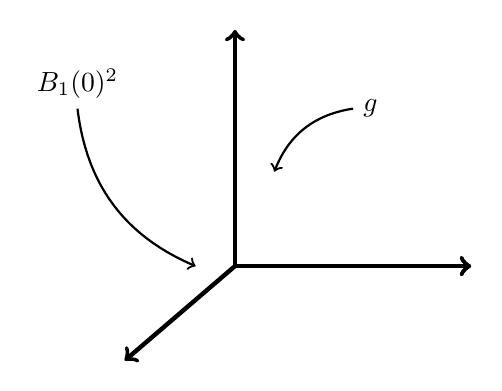
\begin{tikzpicture}
				\hcsphere{-2}{0}{2};
				
				\draw[->,thick] (1.5,2) node[right]{$\graph g$} to[bend right] (.5,1.2);
				\draw[->,thick] (-2,2) node[above]{$B_1(0)\sbs\R^2$} to[bend right] (-.5,0);
				\draw[->,ultra thick] (0,0)--(3,0);
				\draw[->,ultra thick] (0,0)--(0,3);
				\draw[->,ultra thick] (0,0)--(3,0);
				\draw[->,ultra thick] (0,0)--(-1.4,-1.2);
				\end{tikzpicture}
			\end{minipage}
			\medskip\\
			Allgemein möchte man eine (Hyper-) Fläche der Form $ M = \{ X,Y \in \R^{k+m} \mid f(x,y) = 0\}$ lokal als Graph einer Funktion $ x \to g(x) \in \R^m $ schreiben, also $ (x, g(x)) \in M$.
	\begin{center}
		\fbox{
		\begin{minipage}{.4\textwidth}
			\vspace{.4\textwidth}
			Grafik folgt in Kürze.
			\vspace{.4\textwidth}
		\end{minipage}
		}
	\end{center}
	\begin{theorem}[implizite Funktionen]
		Seien $k, m \in \N, \: \Omega \sbs \R^{k + m}$ eine offene Menge und \\$f \in C^1 (\Omega, \R^m)$. Es gebe ein $(\xi, \eta) \in \Omega$ mit $f( \xi, \eta) = 0 $ und $ \det D _y( \xi, \eta) \neq 0$, wobei \\$D _y f(x,y) = \left(\frac{\del f_j}{\del y_l}(x,y)\right)_{j,l = 1, \dots, m}$.\\
		Dann gibt es offene Umgebungen $U \sbs \R$ von $\xi$ und $V \sbs \R^m$ von $\eta$ und ein $\phi \in C^1(U,V)$ mit
		\begin{align*}
		&\{(x,y) \in U \times V \mid f(x,y) =0 \} = \{(x, \phi(x)) \mid x \in U \} \text{ und} \\
		& D  \phi (x) = - ( D _y f(x, \phi(x)))^{-1} D _x f(x,\phi(x)) \forall x \in U
		\end{align*}
	\end{theorem}
	
	\begin{proof}
		Wir definieren $ F \colon \Omega \to \R^{k + m}$ durch 
		\begin{equation*}
		F(x,y) = (\uarrow{\in \R^k}{x}, \underbrace{f(x,y)}_{\in \R^m})
		\end{equation*}
		und erhalten $D F(x,y) = \begin{pmatrix} \mathds{1}_{k \times k} & 0 \\ D_x f(x,y) & D_y f(x,y) \end{pmatrix}$.\\
		Insbesondere ist $\det D F(\xi, \eta)  = \underbrace{(\det \mathds{1}_{k \times k})}_{=1} \underbrace{(\det D_y f(\xi, \eta))}_{\neq 0}$ also $D F(\xi, \eta) \in \mathrm{GL}(k+m)\footnotemark$
		\footnotetext{Menge der invertierbaren $(k+m) \times (k+m)$-Matrizen, \emph{general linear group}}.
		
		Nun erhalten wir aus \emph{Satz 2} offene Mengen $\mc{W}, \wt{\mc{W}} \sbs \R^{k+m}$ mit $(\xi, \eta) \in \mc{W}, \: F(\xi, \eta) \in \wt{\mc{W}}$, sodass $F|_{\mc{W}}$ ein Diffeomorphismus $\mc{W} \to \wt{\mc{W}}$ liefert. Durch verkleinern von $\mc{W}$ (ohne Ändern der Notation, betrifft auch $\wt{\mc{W}}$) können wir $\mc{W} = U \times V $ annehmen wobei $U$ und $V$ offene Umgebungen von $\xi$ bzw. $\eta$ sind.
		\begin{center}
			\fbox{
				\begin{minipage}{.4\textwidth}
					\vspace{.4\textwidth}
					Grafik folgt in Kürze.
					\vspace{.4\textwidth}
				\end{minipage}
			}
		\end{center}
		Weiter setzen wir $G = ( F|_{\mc{W}})^{-1} \colon \wt{\mc{W}} \to \mc{W}$.\\
		Wegen $F(x,y) = (x,f(x,y))\ \forall(x,y) \in \Omega \supset U \times V$ gibt es eine Funktion $g \colon \wt{\mc{W}} \to V$ mit 
		\begin{align*}
		G(\tilde{x},\tilde{y}) &= (\tilde{x}, g(\tilde{x},\tilde{x})) \quad\forall (\tilde{x},\tilde{y}) \in \wt{\mc{W}} \\
		f(\tilde{x},g(\tilde{x},\tilde{y})) &= \tilde{y} \quad\forall(\tilde{x},\tilde{y}) \in \wt{\mc{W}} \\
		g(x,f(x,y)) &= y \quad\forall (x,y) \in \mc{W} = U \times V
		\end{align*}
		Wegen $(\xi, 0) = (\xi, f(\xi, \eta)) = F(\xi, \eta) \in \wt{\mc{W}}$ erhalten wir nach verkleinern von $U$ ($\mc{W}$ bleibt unverändert, $U$ nach wie vor offene Umgebung von $\xi$) $F(U \times \{0\}) \sbs \wt{\mc{W}}$, insbesondere ist $g(x,0) \: \forall x \in U$ definiert. Für alle $(x,y) \in U \times V$ gilt nun
		\begin{equation*}
		f(x,y) \iff F(x,y) = (x,0) \iff (x,y) = G(x,0) = (x,g(x,0)) \iff y = g(x,0)
		\end{equation*}
		Mit der Definition $\phi \colon U \to V, \: x \to g(x,0)$, ergibt sich \[f(x,y) = 0 \iff y = \phi (x) \: \forall (x,y) \in U \times V.\]
		Da $G$ ein Diffeomorphismus ist, folgt $g \in C^1 (\wt{\mc{W}}, V)$ und $\phi \in C^1 (U,V)$. Mit der Kettenregel erhalten wir $f(x, \phi(x)) \: \forall x \in U = 0 \rightarrow D _x f(x,\phi(x)) + \underbrace{D _y f(x, \phi(x))}_{\mathclap{\text{invertierbar wegen Umkehrsatz}}} D  \phi(x) = 0$. \\
		\end{proof}
		Grundkonzepte der Untermannigfaltigkeiten. Mannigfaltigkeiten „sehen lokal so aus“ wie eine Umgebung im $\R^k$ für ein $ k \in \N$.
		
		\begin{defin}[Immersion]
			Sei $\Omega \sbs \Rn$ nichtleer und offen, $\phi \in C^1(\Omega, \R^m), \: m \geq n$.\\ Die Abbildung $\phi$ heißt \emph{Immersion}, falls der Rang von D$\phi(x) \: \forall x \in \Omega$ stets minimal ist (also gleich $n$).\\
			(Alternativ: $D\phi(x) \colon \Rn \to \R^m$ ist (linear und) injektiv.)
		\end{defin}
		
		\begin{defin}[Untermannigfaltigkeit]
			Seien $m,n \in \N \cup \{0\}, \: m \leq n$.\\
			Eine \emph{$C^1$-Untermannigfaltigkeit des $\Rn$ mit Dimension $m$} (kurz: \emph{Mannigfaltigkeit}) ist eine nichtleere Menge $M \sbs \Rn$ (Notation $M^m$) mit der folgenden Eigenschaft:\\
			Für jedes $\xi \in M$ existiert eine offene Umgebung $\Omega \sbs \Rn, \: \xi \in \Omega$, eine (offene) Menge $U \sbs \R^m$ und eine Immersion $\phi \in C^1(U,\Rn),$ die $U$ homöomorph auf $\image\phi = M \cap \Omega$.\medskip\\
			\begin{minipage}{\textwidth}
				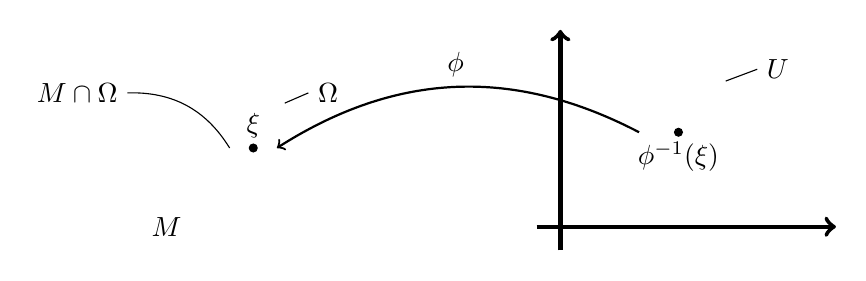
\begin{tikzpicture}
				\saucer{0}{0}{1};
				
				\draw (1,1.7) node[left]{$M \cap \Omega$} to[bend left] (2.3,1);
				\draw (3.3,1.7) node[right]{$\Omega$} to (3,1.57);
				\node at (1.5,0) {$M$};
				\filldraw (2.6,1) circle[radius=.05] node[above]{$\xi$};
				
				\draw[->,thick] (7.5,1.2) to[bend right] node[above]{$\phi$} (2.9,1);
				
				\draw[->,ultra thick] (6.2,0)--(10,0);
				\draw[->,ultra thick] (6.5,-.3)--(6.5,2.5);
				\squigglyset{7}{.4}{1.3}{.7};
				\filldraw (8,1.2) circle[radius=.05] node[below]{$\phi^{-1}(\xi)$};
				\draw (9,2) node[right]{$U$} to (8.6,1.85);
				\end{tikzpicture}
			\end{minipage}\medskip\\
			Die Abbildung $\phi$ heißt \emph{(lokale) Parametrisierung von $M$ um $\xi$}, ihre Umkehrung $\phi \colon M\cap\Omega \to U$ bzw. das Paar $(\phi^{-1},U)$ heißt \emph{Karte} und eine Familie von Karten, deren Urbilder ganz $M$ überdecken, bildet einen \emph{Atlas}.
		\end{defin}
	
	
\end{document}